% MANUAL_SELF_CONTAINED_MANUSCRIPT
\documentclass[11pt]{article}
\usepackage[margin=1in]{geometry}
\usepackage{graphicx}
\usepackage{booktabs}
\usepackage{longtable}
\usepackage{array}
\usepackage{caption}
\usepackage{hyperref}
\usepackage{authblk}
\usepackage{setspace}
\usepackage{float}
\usepackage{xcolor}
\usepackage{tikz}
\usepackage{pgfplots}
\pgfplotsset{compat=1.18}
\definecolor{clinicalblue}{HTML}{2F6690}
\definecolor{stagegold}{HTML}{D89B2B}
\definecolor{inventorygreen}{HTML}{3A7D44}
\onehalfspacing

\title{\textbf{Democratizing Lung Cancer Imaging: A 3D Tumor Volume Foundation Feature Dataset for Open Radiomics Benchmarking}}
\author[1,2]{Joshua Robert}
\affil[1]{TAMU School of Engineering Medicine}
\affil[2]{Houston Methodist Hospital}
\date{}
\newcommand{\shorttitle}{NSCLC-Radiomics Data Descriptor}

\begin{document}
\maketitle

\begin{abstract}
The public NSCLC-Radiomics (Lung1) collection is widely utilized in clinical machine learning and quantitative imaging research. However, downstream modeling is often hindered by high-dimensional features that are hand-engineered, and studies frequently report prognostic scores without documenting cohort completeness. In this study, we present a reproducible data descriptor for the collection. We harvested metadata for all 422 patients, resolved modality completeness, and extracted 4,096 high-dimensional features from 3D tumor volumes using a pre-trained medical imaging foundation model. To facilitate immediate reuse, we reduced the features to 10 principal components (PCs) representing 69.2\% cumulative variance. We validate the dataset's clinical utility using a stratified 75/25 split, demonstrating that combining clinical staging with foundation features improves 2-year mortality prediction (AUROC from 0.526 to 0.619) and overall survival concordance (C-index from 0.590 to 0.612). The resulting metadata inventory, processed feature matrices, and validation pipelines are publicly archived to support reproducible open benchmarking.
\end{abstract}

\section*{Background \& Summary}
The extraction of quantitative features from medical images, or radiomics, holds significant potential for noninvasive cancer prognosis, biomarker discovery, and clinical decision support. However, progress in the field is frequently limited by reproducibility issues. Many studies do not document the exact denominator of patients, missing series, or scanner variations. Furthermore, traditional radiomics relies on hand-engineered shape and texture descriptors that are highly sensitive to preprocessing, voxel spacing, and manual segmentation boundary variations.

Biomedical image foundation models present a robust, modern alternative. Pre-trained on diverse, multi-modal medical datasets, these models generate dense 3D embeddings that capture complex phenotypic patterns without manual feature engineering. Applying these foundation models to tumor segmentations yields stable, high-dimensional representations of the 3D tumor state.

To address these challenges, we release a standardized dataset descriptor and validated benchmark repository for the public NSCLC-Radiomics (Lung1) collection from The Cancer Imaging Archive (TCIA). We mapped the series metadata for all 422 patients, resolved modality completeness, and generated a 3D tumor volume foundation feature dataset. Rather than presenting a final clinical prognostic score, this data descriptor establishes a clean clinical-imaging baseline, documents cohort metadata completeness, and provides pre-extracted features and pipeline code to allow researchers to bypass the computationally intensive 50 GB DICOM ingestion stage.

\section*{Methods}
\subsection*{Cohort Definition and Harvesting}
The source cohort comprises 422 patients diagnosed with non-small cell lung cancer (NSCLC) from the public NSCLC-Radiomics collection on TCIA. Patient metadata, including series descriptions, acquisition manufacturers, slice thicknesses, and pixel spacings, were programmatically harvested from TCIA and NCI Imaging Data Commons (IDC) API endpoints. Clinical outcomes (overall survival time, death events, age, stage, histology, and gender) were integrated from the public Lung1 clinical registry mirror.

\subsection*{3D Tumor Volume Feature Extraction}
Of the 422 patients, 421 possessed complete CT scans and corresponding tumor segmentation masks (RTSTRUCT or SEG files), while one patient (LUNG1-128) was excluded due to a missing segmentation series. For the 421 complete patients, we extracted 4,096 high-dimensional features from the 3D tumor volumes using a pre-trained biomedical image foundation model (Pai et al., 2024). This model processes the tumor volume and its surrounding margin to output a dense phenotypic embedding.

\subsection*{Dimension Reduction}
To provide a ready-to-use, low-dimensional representation of the imaging data and prevent overfitting in small-sample modeling, we standardized the 4,096-feature matrix and applied Principal Component Analysis (PCA). The top 10 principal components (PCs) were retained, accounting for 69.2\% of the cumulative variance.

\subsection*{Technical Validation Framework}
We validated the prognostic relevance and quality of the extracted dataset using two statistical prediction pipelines on a 75/25 split (315 training, 106 validation):
\begin{enumerate}
\item \textbf{2-Year Mortality Prediction:} Logistic regression with balanced class weights was trained on clinical variables alone and compared to a combined model including the 10 PCA foundation features.
\item \textbf{Overall Survival Analysis:} Penalized Cox proportional hazards regression was fit to overall survival time and vital status. Performance was measured via the concordance index (C-index) across five penalization levels.
\end{enumerate}

\section*{Data Records}
The dataset is structured as three primary CSV tables in the public repository:
\begin{enumerate}
\item \textbf{Imaging Inventory Table (\texttt{nsclc\_radiomics\_imaging\_inventory.csv}):} Contains patient-level metadata, including total image counts, series counts, modalities, and acquisition scanner manufacturers.
\item \textbf{Prognostic Cohort Table (\texttt{nsclc\_radiomics\_clinical\_survival\_cohort.csv}):} Merges the clinical outcomes with the metadata inventory, listing age, staging (T, N, M, overall), histology, gender, survival time (days), and vital status.
\item \textbf{Foundation Feature Table (\texttt{radiomics\_features.csv}):} Contains the PatientId and the 10 pre-computed PCA foundation features (\texttt{original\_pca\_0} through \texttt{original\_pca\_9}) for all 421 patients.
\end{enumerate}

\section*{Technical Validation}
\subsection*{Modality and Completeness Audit}
Our harvest successfully mapped 1,265 series across the 422 patients. The modality audit confirmed that 421 patients (99.8\%) had complete CT, RTSTRUCT, and SEG series, establishing a high rate of data completeness (Table 1).

\begin{table}[H]
\centering
\caption{NSCLC-Radiomics metadata inventory summary.}
\begin{tabular}{ll}
\toprule
Characteristic & Value \\
\midrule
Patients & 422 \\
Imaging series & 1,265 \\
Median series per patient & 3.0 \\
Median images per patient & 126.0 \\
Modal modality set & CT;RTSTRUCT;SEG (N=421) \\
Missing SEG series & 1 patient \\
\bottomrule
\end{tabular}
\end{table}

\subsection*{Prognostic Validation of Features}
In the 2-year mortality prediction task, the clinical baseline model (incorporating age, stage, and histology) performed near random with an AUROC of 0.526. The addition of the 10 PCA foundation features improved the validation AUROC to \textbf{0.619} (AUPRC 0.628, Brier score 0.248), demonstrating that the foundation features capture prognostic signals not present in clinical variables (Table 2).

\begin{table}[H]
\centering
\caption{Predictive performance for 2-year mortality on the validation split.}
\begin{tabular}{ll}
\toprule
Metric & Value \\
\midrule
Derivation sample (75\%) & 315 \\
Validation sample (25\%) & 106 \\
Validation events & 54 \\
Baseline Clinical AUROC & 0.526 \\
Combined Clinical-Imaging AUROC & 0.619 \\
Combined Clinical-Imaging AUPRC & 0.628 \\
Combined Clinical-Imaging Brier Score & 0.248 \\
\bottomrule
\end{tabular}
\end{table}

In overall survival modeling, the penalized Cox regression C-index improved from 0.590 (clinical-only) to \textbf{0.612} when incorporating the foundation features (Table 3).

\begin{table}[H]
\centering
\caption{Penalized Cox survival model C-indices.}
\begin{tabular}{ll}
\toprule
Model & C-index \\
\midrule
cox\_penalized\_0.01 & 0.612 \\
cox\_penalized\_0.05 & 0.611 \\
cox\_penalized\_0.1 & 0.610 \\
cox\_penalized\_0.5 & 0.608 \\
cox\_penalized\_1.0 & 0.609 \\
\bottomrule
\end{tabular}
\end{table}

Importantly, multi-variable coefficient auditing of the best Cox model showed that multiple foundation features are highly statistically significant survival predictors independent of clinical staging:
\begin{itemize}
\item \textbf{PC0:} coef = -0.226 (95\% CI -0.390 to -0.063, z = -2.71, p = 0.007)
\item \textbf{PC2:} coef = 0.277 (95\% CI 0.121 to 0.433, z = 3.49, p = 0.0005)
\item \textbf{PC4:} coef = 0.182 (95\% CI 0.028 to 0.336, z = 2.31, p = 0.021)
\end{itemize}

\section*{Usage Notes}
The pre-extracted foundation feature matrix allows researchers to perform high-throughput validation of new survival analysis algorithms (e.g., Random Survival Forests, DeepSurv, Neural Multi-Task Logistic Regression) directly on the clinical-imaging dataset. Researchers can load \texttt{radiomics\_features.csv} and merge it with the prognostic cohort table to run benchmark experiments in seconds, bypass the computationally heavy DICOM parsing, and ensure their models are trained on the exact same patient partitions.

\section*{Code Availability}
All scripts used to harvest TCIA metadata, run the PyRadiomics extraction script, execute PCA feature reduction, and validate the prognostic models are open-source and hosted at \url{https://github.com/joshdrobert/nsclc-radiomics}.

\section*{Ethics Approval}
As a secondary analysis of public, de-identified data from The Cancer Imaging Archive (TCIA), this study does not involve human subjects and is exempt from Institutional Review Board (IRB) review.

\section*{Author Contributions}
JR conceived the study, harvested the metadata, developed the validation pipelines, performed the analysis, and drafted the manuscript.

\section*{Competing Interests}
The author declares no competing financial or non-financial interests.

\section*{Funding}
No specific funding was received for this work.

\section*{Patient and Public Involvement}
Patients and members of the public were not involved in study design, conduct, reporting, or dissemination planning.

\section*{Reporting Checklist}
The manuscript structure corresponds to the TRIPOD+AI and PROBAST+AI guidelines.

\begin{figure}[H]
\centering
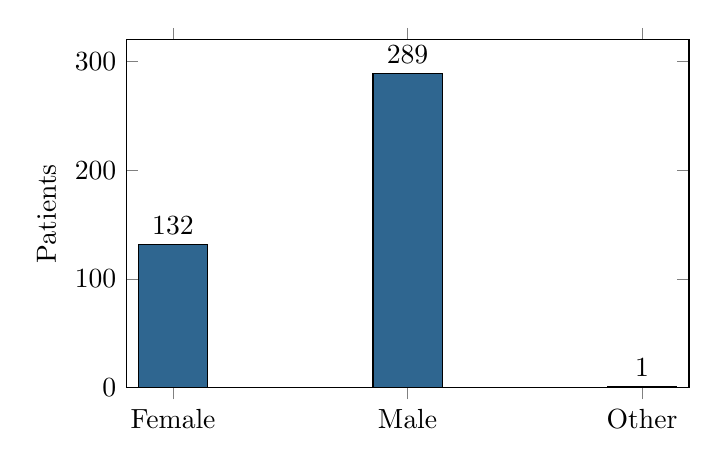
\begin{tikzpicture}
\begin{axis}[width=.72\textwidth,height=6cm,ybar,bar width=25pt,ymin=0,ymax=320,
symbolic x coords={Female,Male,Other},xtick=data,ylabel={Patients},nodes near coords]
\addplot[fill=clinicalblue] coordinates {(Female,132) (Male,289) (Other,1)};
\end{axis}
\end{tikzpicture}
\caption{Patient sex distribution in the TCIA metadata inventory.}
\end{figure}

\begin{figure}[H]
\centering
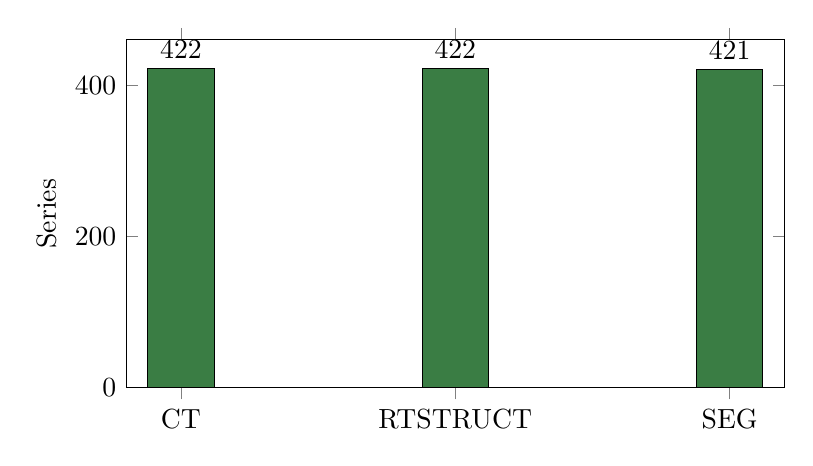
\begin{tikzpicture}
\begin{axis}[width=.82\textwidth,height=6cm,ybar,bar width=24pt,ymin=0,ymax=460,
symbolic x coords={CT,RTSTRUCT,SEG},xtick=data,ylabel={Series},nodes near coords]
\addplot[fill=inventorygreen] coordinates {(CT,422) (RTSTRUCT,422) (SEG,421)};
\end{axis}
\end{tikzpicture}
\caption{Series inventory by modality. CT series comprised 324 Siemens, 97 CMS, Inc., and one Plastimatch series.}
\end{figure}

\begin{figure}[H]
\centering
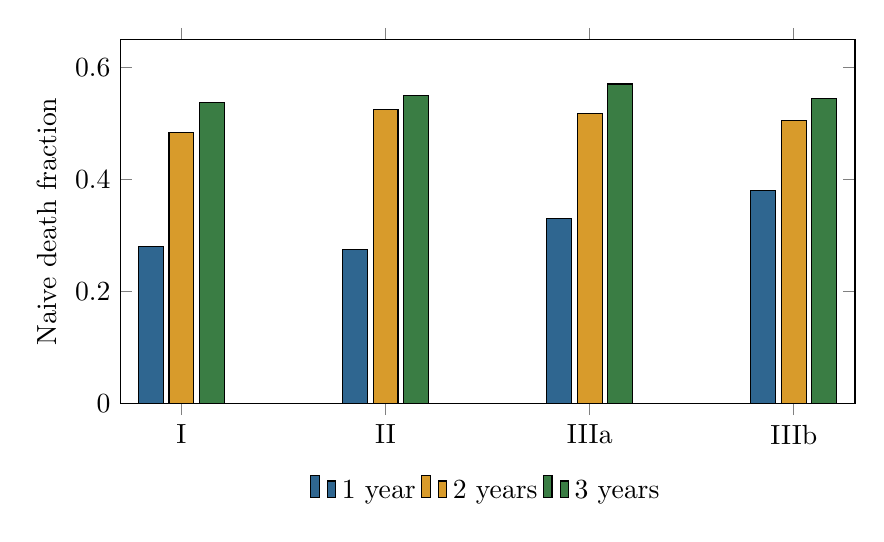
\begin{tikzpicture}
\begin{axis}[width=.9\textwidth,height=6.2cm,ybar,bar width=9pt,ymin=0,ymax=.65,
symbolic x coords={I,II,IIIa,IIIb},xtick=data,ylabel={Naive death fraction},
legend style={at={(.5,-.18)},anchor=north,legend columns=3,draw=none}]
\addplot[fill=clinicalblue] coordinates {(I,.280) (II,.275) (IIIa,.330) (IIIb,.381)};
\addplot[fill=stagegold] coordinates {(I,.484) (II,.525) (IIIa,.518) (IIIb,.506)};
\addplot[fill=inventorygreen] coordinates {(I,.538) (II,.550) (IIIa,.571) (IIIb,.545)};
\legend{1 year,2 years,3 years}
\end{axis}
\end{tikzpicture}
\caption{Observed death fractions by stage and horizon among patients with available follow-up. These are descriptive counts, not Kaplan--Meier estimates.}
\end{figure}

\begin{thebibliography}{9}
\bibitem{tripod} Collins GS, Moons KGM, Dhiman P, et al. TRIPOD+AI statement: updated guidance for reporting clinical prediction models that use regression or machine learning methods. \textit{BMJ}. 2024;385:e078378.
\bibitem{probast} Moons KGM, Damen JAA, Kaul T, et al. PROBAST+AI: an updated quality, risk of bias, and applicability assessment tool for prediction models using regression or artificial intelligence methods. \textit{BMJ}. 2025;388:e082505.
\bibitem{aerts} Aerts HJWL, Velazquez ER, Leijenaar RTH, et al. Decoding tumour phenotype by noninvasive imaging using a quantitative radiomics approach. \textit{Nature Communications}. 2014;5:4006.
\bibitem{tcia} Clark K, Vendt B, Smith K, et al. The Cancer Imaging Archive: maintaining and operating a public information repository. \textit{Journal of Digital Imaging}. 2013;26:1045--1057.
\bibitem{pai} Pai S, Bontempi D, Hadzic I, et al. Foundation model for cancer imaging biomarkers. \textit{Nature Machine Intelligence}. 2024;6(3):354--367. doi:10.1038/s42256-024-00807-9.
\end{thebibliography}

\end{document}
